\RequirePackage{amsmath}
\documentclass[runningheads]{llncs}
\usepackage[utf8]{inputenc}
\usepackage{graphicx}
% \usepackage{amsmath}
\usepackage{amsfonts}
\usepackage{amssymb}
\usepackage{diagbox}
\usepackage{booktabs}
\usepackage{multirow}
\usepackage[caption = false]{subfig}
% \usepackage[english,main=spanish]{babel}
% If possible, figure files should be included in EPS format.
%
% If you use the hyperref package, please uncomment the following line
% to display URLs in blue roman font according to Springer's eBook style:
% \renewcommand\UrlFont{\color{blue}\rmfamily}

\begin{document}
%
\title{Cross-cultural image-based author profiling\\ in Twitter}

%\titlerunning{Abbreviated paper title}
% If the paper title is too long for the running head, you can set
% an abbreviated paper title here

\author{Ivan Feliciano \and
Second Author \and
Third Author}
%
\authorrunning{I. Feliciano et al.}
% First names are abbreviated in the running head.
% If there are more than two authors, 'et al.' is used.
%
\institute{Instituto Nacional de Astrofísica, Óptica y Electrónica\\
\email{ivan.felavel@gmail.com}\\
}

\maketitle

\begin{abstract}

Current approaches have shown that it is possible to use information extracted from images to solve gender identification. These proposals addressed the problem by using data from users of the same language, e.g. they employ shared images of English language registered users to train their models and test over a set of images from users of English language. Despite the good results, the information from users of some languages is not always available. In this work we present a cross-cultural approach where we show that individuals with similar demographic aspects event though from different dialects and cultures usually share likewise images. We show that we can improve or preserve the effectiveness of a model with a monolingual perspective by taking advantage of a dataset from another language. We also analyzed some high level features obtained from the images that helped to make gender prediction and are also useful among the different languages.
\keywords{author profiling \and cross-cultural\and image-based \and gender prediction.}
\end{abstract}

\section{Introduction}

The shared content on social networks includes information in different modalities such as text, images, audio and video.
All this data can be used to extract valuable information from users.
Author profiling (AP) is the analysis of shared content in order to predict different attributes of authors such as gender, age, personality, native language, or political orientation \cite{rangel_rosso_montes-y-gomez_potthast_stein}.
Determination of such aspects can be applied in a wide variety of fields, for instance, gender and age identification have been
used in marketing and legal investigation \cite{miller_dickinson_hu_2012}. From a forensic perspective, in many crime 
cases, the culprits hide their real identities to avoid being detected \cite{cheng_chandramouli_subbalakshmi_2011}. Similarly, from
a marketing point of view, gender identification is useful
for companies to be able to know if a product is of interest
to a demographic \cite{rangel2013use}.

The most common approach to tackle the author profiling task
is analyzing text written by authors. 
For example, \cite{cheng_chandramouli_subbalakshmi_2011}, \cite{FATIMA2017886} and \cite{gomez2016improving}
have used text shared in social networks to 
classify authors by gender and age.
Besides these text-based perspectives,
some other works like \cite{merler2015you} and 
recently the PAN 2018 AP task \cite{rangel_rosso_montes-y-gomez_potthast_stein}  aim
for a gender identification from a multimodal standpoint
where in addition to text, images as source of information
are included.

The proposals mentioned above have shown that it is possible to use information extracted from images to solve gender identification. However, they addressed the problem by using data from users of the same language, e.g. they employ shared images of English language registered users to train their models and test over a set of images from users of English language. Despite the good results, 
the information from users of some other languages is not always available.
Starting from this, the inquisitiveness to know if shared images on social media are to a certain extent independent of the language of the users motivated us to do this research.

In this work we present a cross-cultural approach where we show that individuals with similar demographic aspects even though from different dialects and cultures usually share likewise images.
For instance, from the results of Section \ref{section:results},
we can confirm some obvious and stereotypes assumptions remain
between different languages. For example, men share more content related to sports.
% Men share more content related to sports and women share more images related to clothes and makeup.

To meet our cross-cultural approach
% we employ the collection provided by the 
% the PAN 2018 AP task. This dataset is 
% grouped by user language, there are three
% languages; English, Spanish and Arab. Each
% group is composed of text and image tweets.
% We only focus on using the images. Through the extraction of semantic features of 
we employ images from Twitter. Through the extraction of semantic features of 
the images shared by the authors, several models
were trained and tested. Using a monolingual approach, some of these models
were trained and tested using the data of users
of the same language. The rest of the models 
were trained adding the collections of the 
other languages and evaluated with user data 
whose language is not necessarily in the 
training collections. The best model was achieved using as our training set the union of all collections. 

Our main contribution is the confirmation
that for the task of gender identification, 
% images from social media are independent
the size of the data matters more than the
language of the users. We show that we can improve the effectiveness of a model with a monolingual perspective by taking advantage of a larger dataset from another language. We also analyzed some high level features obtained from the images that helped to make gender prediction and are also useful among the different languages.

\section{Related work}

A significant amount of work has been done for the problem of inferring gender, focusing on
textual analysis. However, nowadays content in image format is very popular and 
very little attention has been paid although the text-based approach has limitations like it requires to develop a particular model for every language in a set of these \cite{ciot2013gender}.

Recent works have shown the possibility of use visual content
to predict the gender of the users. 
Often the visual information that is used are the images shared in the user's feed, 
however, in \cite{merler2015you}, they employ three different sources: profile pictures, images from the feed,
and profile color patterns.
The authors in \cite{you2016picture} use a Bag of Visual Words model
and image tags from Pinterest generated by the users. Both research works
take on data from english-speaking users.

Lately, the Author Profiling shared task at PAN 2018 had as goal, 
gender identification from a multimodal perspective, where texts and images were 
given and they cover three languages: arab, english and spanish.
The participants used different approaches to solve the problem,
where the solutions that involved deep learning techniques were the most outstanding.
In a very general way, with respect to gender classification based only on images, we can lump
together three approaches: based on face recognition, based on pre-trained models
and based on basic image processing techniques as color histograms.

The most prominent results were from the second approach \cite{rangel_rosso_montes-y-gomez_potthast_stein}. The authors in 
\cite{aragon2018straightforward}, 
\cite{takahashi_tahara_nagatan_miura_taniguchi_ohkuma} and \cite{sierra_gonzales}
used as feature extractor, with a different level of abstraction, the
VGG16 deep network \cite{zisserman_simonyan_2015}.
% These previous works only indicate their results from a monolingual perspective.

Our proposal follows the same scheme as \cite{aragon2018straightforward}, 
where each author is represented with one average vector that contains
information from all the images that were passed through the VGG16 network.
This vector is a probability distribution over one thousand categories
comprising objects and scenes in every image. Finally, the vector is the input to a model that predicts gender.

% La propuesta de este trabajo sigue el mismo esquema que \cite{aragon2018straightforward}, donde utiliza el vector generado por la capa de salida. Este vector es una
% distribución de probabilidad sobre mil categorías, compuestas por 
% objetos y escenas que puede contener la imagen. Como cada autor cuenta 
% con diez tuits de imágenes, se obtiene un vector promedio para 
% representar a cada usuario y éste es utilizado sobre otro modelo para 
% clasificar entre dos Genders: Male y Female. 
% Los trabajos anteriores, sólo indican los resultados de la evaluación de los modelos de clasificación con un enfoque monolingüe. 
% % , donde \cite{sierra_gonzales} adicionalmente usó ResNet50 \cite{7780459} para comparar resultados, obteniendo mejores resultados con la última.

% En la tarea del PAN 2018 los participantes identificaron el Gender
% de usuarios de Twitter a través de una perspectiva multilingüe y multimodal. Los participantes utilizaron diferentes enfoques para resolver la tarea,
% donde las soluciones predominantes aplicaron técnicas de aprendizaje profundo.
% Los enfoques para la clasificación de imágenes se pueden agrupar en tres tipos:
% \begin{enumerate}
%     \item Basado en reconocimiento de rostros.
%     \item Basados en modelos pre-entrenados y herramientas de procesamiento de
%     imágenes como ImageNet.
%     \item Características extraídas ``a mano'' como histogramas de color y bolsas 
%     de palabras visuales.
% \end{enumerate}

% Respecto al segundo tipo de enfoque, los mejores resultados se obtuvieron 
% con la extracción de características semánticas a partir de las 
% imágenes \cite{rangel_rosso_montes-y-gomez_potthast_stein}.
% Los mejores resultados para la clasificación usando imágenes los obtuvieron los
% autores en \cite{takahashi_tahara_nagatan_miura_taniguchi_ohkuma}, quienes utilizaron 
% un modelo pre-entrenado de red neuronal convolucional (CNN por sus siglas en inglés) 
% basado en ImageNet. Algunos de los autores en los primeros puestos como \cite{aragon2018straightforward}, 
% \cite{takahashi_tahara_nagatan_miura_taniguchi_ohkuma} y \cite{sierra_gonzales} utilizaron como modelo, para la extraccón de características, la red VGG16 \cite{zisserman_simonyan_2015}, donde \cite{sierra_gonzales} adicionalmente usó ResNet50 \cite{7780459} para comparar resultados, obteniendo mejores resultados con la última.

% La propuesta de este trabajo sigue el mismo esquema que \cite{aragon2018straightforward}, donde utiliza el vector generado por la capa de salida. Este vector es una
% distribución de probabilidad sobre mil categorías, compuestas por 
% objetos y escenas que puede contener la imagen. Como cada autor cuenta 
% con diez tuits de imágenes, se obtiene un vector promedio para 
% representar a cada usuario y éste es utilizado sobre otro modelo para 
% clasificar entre dos Genders: Male y Female. 
% Los trabajos anteriores, sólo indican los resultados de la evaluación de los modelos de clasificación con un enfoque monolingüe. Sin embargo, esta investigación tiene una perspectiva crosslingüe.

% Ap-
% proaches based on face recognition do not belong to the best, which may be rooted inthe fact that many images do not show faces—and if, the contained faces do not depict
% the author.
% \begin{itemize}
%     \item Takahashi, Ezra.
%     \item Buscar qué se ha hecho en escenarios multilingüe.
%     \item Cross lingual pretraining.
%     \item GENDER PREDICTION BASED ON SEMANTIC ANALYSIS OF SOCIAL MEDIA 
%     IMAGES.
% \end{itemize}

\section{Proposed approach}

To be able to show that the shared images are independent of the language
of the authors, we proposed to train classifiers
with different combinations of training data of user images 
in the three languages. After training all the possible models, they
are evaluated with the test set for each language individually.
For example, we can train a learning model using images from spanish-speaking
and english-speaking users. Subsequently, we measure its performance
using images from arab-speaking authors.
Our approach comprises two parts; authors' representation and 
evaluation schemes.

% \subsection{Representation of users}

Generally speaking, we can assume that we possess $N$ images shared
by every user. The representation of each image is extracted from 
a pre-trained convolutional neural network. The used model has as output a probability distribution
over 1000 possible labels. These labels are objects and scenes contained
in a picture.
To get only one feature vector that represents each author, 
we average the vectors of the $N$ images. The average vectors 
are the ones used as inputs for the learning model. Figure \ref{fig:img_representation} shows the above description.

\begin{figure}[ht]
    \centering
    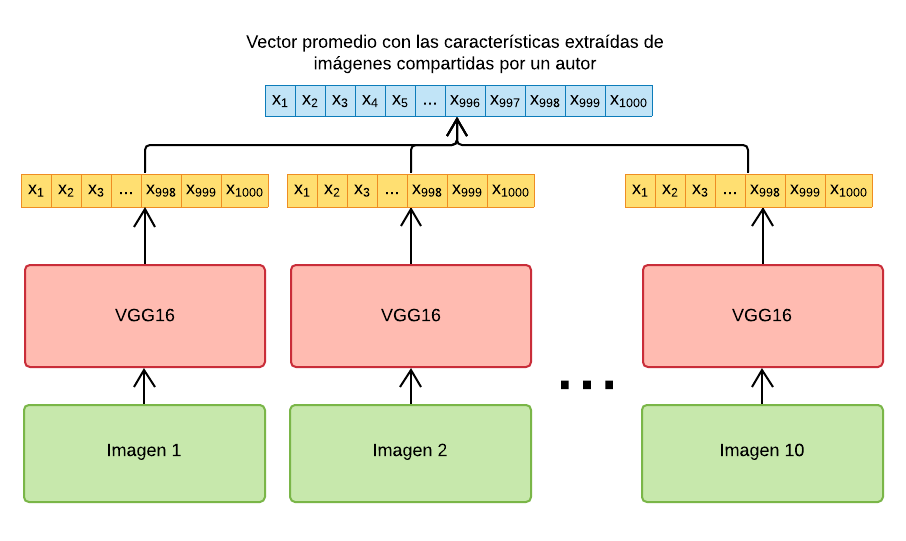
\includegraphics[scale=0.25]{img/features_extraction.png}
    \caption{Representation scheme of one author through the 
    feature extraction of the $N$ shared images.}
    \label{fig:img_representation}
\end{figure}

% \subsection{Evaluation schemes}

For the part of the evaluation schemes, we build one classifier for each subset of the set of the collections from user images in all different languages.
Namely, given a set $\mathbb{X} = \{\text{Arab}, 
\text{Spanish}, \text{English}\}$, where each element
from $\mathbb{X}$ is a collection of user representations
of the respective language, the $i-th$ classifier was trained
with a set $X_i \subseteq \mathbb{X}$ and $X_i \neq \varnothing$.
After every possible classifier training, they are evaluated with a collection 
$Y \in \mathbb{Y}$, where $\mathbb{Y}$ is defined similarly to
$\mathbb{X}$ but with respect to the test sets.
% Figure \ref{fig:classifier} expresses an example of one classifier.
 
% \begin{figure}[ht]
%     \centering
%     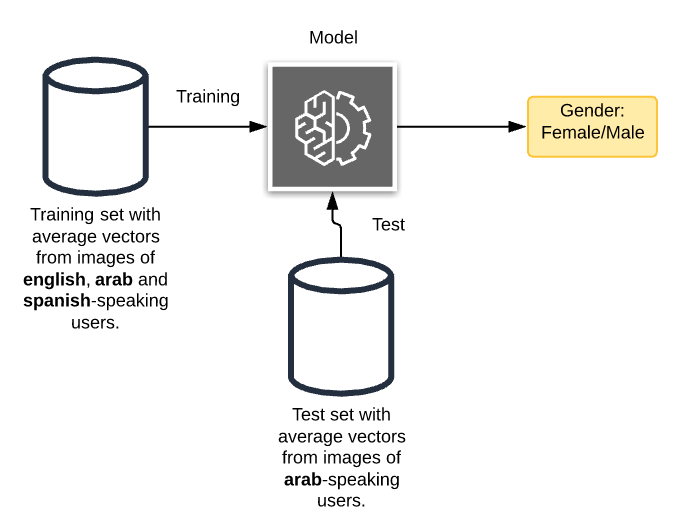
\includegraphics[scale=0.3]{img/classifier_scheme.png}
%     \caption{Pipeline of a classifier trained with images of users 
%     from english, arab and spanish-speaking users and evaluated using
%     the test arab collection.}
%     \label{fig:classifier}
% \end{figure}


\section{Experimental setup}

% Sugiero enfocar la sección 4 en "experimental settings", y en ella
% contar de los datos, de los descriptores de imágenes que usamos (porque
% en teoría podría ser cualquier cosa), del clasificador, de la medida de
% evaluación.

The objective of our experiments is to demonstrate that our
proposed cross-cultural approach take advantage of data from
different languages to classify users in a given tongue.
We do not focus on improving the state of the art results from
other works, but at least improve or preserve the effectiveness of a model with a 
monolingual perspective. For our experiments
we use a collection of images from Twitter provided by the PAN 2018 AP task.
In particular, this collection is grouped by users of three languages (English, 
Spanish, Arab) with ten images per author. The sets are balanced with respect
to gender. Table \ref{table-datasets} describes the collections with regard
number of users and languages.


\begin{table}[]
\centering
\caption{Number of users for each language for training and test sets. There is the same number of women as there are for men.}
\label{table-datasets}
\begin{tabular}{@{}lllll@{}}
\toprule
         & Arab & Spanish & English & Total \\ \midrule
Training & 1500 & 3000    & 3000    & 7500  \\ \midrule
Test     & 1000 & 2200    & 1900    & 5100  \\\midrule
Total    & 2500 & 5200    & 4900    & 12600 \\ \bottomrule
\end{tabular}
\end{table}

To generate the descriptors of the images we use is the VGG16 convolutional
neural network based on ImageNet and we used as machine learning algorithm a support vector 
machine (SVM) with a linear kernel for training and classification. The 
baseline to compare our proposal are monolingual classifiers, i.e. 
those classifiers trained and tested with images from users of the same language.
The metric to compare distinct classifiers performance is the accuracy, the proportion of samples correctly classified.

% \begin{table}[]
% \caption{Number of users for each language for training and test sets. There is the same number of women as there are for men.}\label{table-datasets}
% \centering
% \begin{tabular}{|l|l|l|l|l|}
% \hline
%               & Arab & Spanish & English & Total \\ \hline
% Training & 1500  & 3000    & 3000   & 7500  \\ \hline
% Test       & 1000  & 2200    & 1900   & 5100  \\ \hline
% Total         & 2500  & 4900    & 5200   & 12600 \\ \hline
% \end{tabular}
% \end{table}


% - Ahora no se presentan bien, ni se les saca provecho, los resultados de
% la tabla 4. En esa tabla veo que se presentan 3 tipos de resultados:
% monolingues, crosslingues y monolingues enriquecidos con datos de otros
% lenguajes. Sugiero dos cosas: i) indicar esos 3 tipos de resultados en
% la tabla, agregando una columna extra que los agrupe, ii) en el texto
% explicar cada uno de esos experimentos, y DECIR QUE MUESTRAN LOS
% RESULTADOS.
% - Sugiero hacer una sección 5.1 de Análisis o discusión.

% - Sobre análisis: muy bien lo que has incluido, como materia prima, pero
% no como presentación final. hay que reunirnos a definir qué poner
% exactamente, pero lo que sí veo que hace falta es explicar el objetivo
% atrás de cada análisis. Por ejemplo, yo veo ue podríamos tener dos
% claros objetivos: i) mostrar en cada Language qué ayuda a diferenciar
% entre Males y Females, ii) tratar de mostrar las SEMEJANZAS y
% diferencias por Language. habrá que enfatizar más las semejanzas pues esas
% son el corazón de nuestra idea, sin semejanzas lo crosslingue no
% serviría. Pero claro, viendo que el mejor resultado lo tenemos cuando
% usamos también datos de propio lenguaje en training, entonces hay que
% mostrar también las diferencias.

\section{Results and discussion}\label{section:results}

Table \ref{results_accuracy} reports the evaluation measure 
of every classifier. We grouped together
four types of results: $\mathrm{I}$) monolingual classifiers,
and our cross-cultural approach is splitted in three $\mathrm{II}$) 
$\mathrm{III}$) and $\mathrm{IV}$), where the first ones are evaluated using 
a language that was not used in the training and the last ones are 
those where we add data from languages other than the one used in 
the evaluation. The results highlighted in bold indicate those 
classifiers where each test language obtains its best value in the 
measure of evaluation. We can see that several classifiers achieved 
the same accuracy for the same language. The classifier that reaches
the highest scores for the three languages is the one in $\mathrm{IV}$ where its 
training set is $X_i = \mathbb{X}$, i.e., all the collections are used.
The worst results are those where images from arab-speaking users
are employed to classify english and spanish-speaking users. We 
can assume that it should be because the size of the training data,
the arab dataset is half of the other languages collections.
From this results we are able to make the assumption that
add information regardless of the user's language produces better
classifiers.

\begin{table}[ht]
\centering
\caption{Accuracy for all classifiers.}
\label{results_accuracy}
\begin{tabular}{@{}llll@{}}
\toprule
\multicolumn{1}{c}{Group}        & \multicolumn{1}{c}{$X_i$} & \multicolumn{1}{c}{$Y$} & \multicolumn{1}{c}{Acc} \\ \midrule
\multirow{3}{*}{$\mathrm{I}$)}    & Arab                      & Arab                    & 0.68                         \\
                                 & Spanish                   & Spanish                 & 0.67                         \\
                                 & English                   & English                 & \textbf{0.70}                \\ \midrule
\multirow{6}{*}{$\mathrm{II}$)}   & Arab                      & English                 & 0.63                         \\
                                 &                           & Spanish                 & 0.63                         \\
                                 & Spanish                   & English                 & 0.67                         \\
                                 &                           & Arab                    & 0.70                         \\
                                 & English                   & Spanish                 & 0.67                         \\
                                 &                           & Arab                    & 0.69                         \\ \midrule
\multirow{12}{*}{$\mathrm{III}$)} & Arab Spanish              & English                 & 0.68                         \\
                                 &                           & Spanish                 & 0.67                         \\
                                 &                           & Arab                    & \textbf{0.71}                \\
                                 & Arab English              & English                 & 0.68                         \\
                                 &                           & Spanish                 & 0.66                         \\
                                 &                           & Arab                    & 0.69                         \\
                                 & Spanish English           & English                 & \textbf{0.70}                \\
                                 &                           & Spanish                 & \textbf{0.68}                \\
                                 &                           & Arab                    & 0.70                         \\ \midrule
\multirow{3}{*}{$\mathrm{IV}$)} & Arab Spanish English      & English                 & \textbf{0.70}                \\
                                 &                           & Spanish                 & \textbf{0.68}                \\
                                 &                           & Arab                    & \textbf{0.71}                \\ \bottomrule
\end{tabular}
\end{table}
\subsection{Content extracted from images}
We now analyze the features extracted from the images. These
are based in the image content, i.e. objects and scenes that
are predicted by the VGG16 pre-trained model.
The main objectives of this analysis are: i) show in each language the attributes that helps distinguish between men and women, and ii) show the similarities
and differences among the content shared in the distinct languages.

First, we get a normalized sum vector for each gender in every language.
%The sum vectors are just the sum of feature vectors for 
%every user, grouped by gender. 
In a very rough way
this vector is  analogous to a vector of frequencies.
Attributes with higher values indicate more common labels.
Figure \ref{img-vgg16-freqs} shows those attributes that are
in the intersection of the top 50 of the most frequent labels for every
language and gender.
% the 50 attributes with the highest sum values for every gender and language.


Figure \ref{img-vgg16-freqs} indicates that some attributes
are common between each demographic group. For instance,
some of these features are: web site, book jacket, envelope, comic book and menu. Contrary to the similarities, there are 
some features that are not present in the opposite 
gender in each language.
For example, the difference between the set of most common females features and the set of most common male features is given by:
sunglasses,
pajama, fur coat, theater curtain, cloak, miniskirt, brassiere, hair spray, Band Aid, stole and gown. On the other hand, only men have: 
Windsor tie,
soccer ball, ballplayer, rugby ball, scoreboard, shoe shop, military uniform and basketball.

% For example, for the english
% language, words like 
% ballplayer} and basketball} 
% are in the word cloud of men and miniskirt} and
% pajama} are in the set of women. 
% The intersection of the generated sets
% for men of all the languages are the next terms:
% rugby ball, ballplayer, basketball, and soccer ball}.
% On the other hand the intersection of women image labels
% are: stole, gown, miniskirt, fur coat, brassiere} and pajama}.

\begin{figure}[h]
\centering
\subfloat[Females most frequent attributes. ]{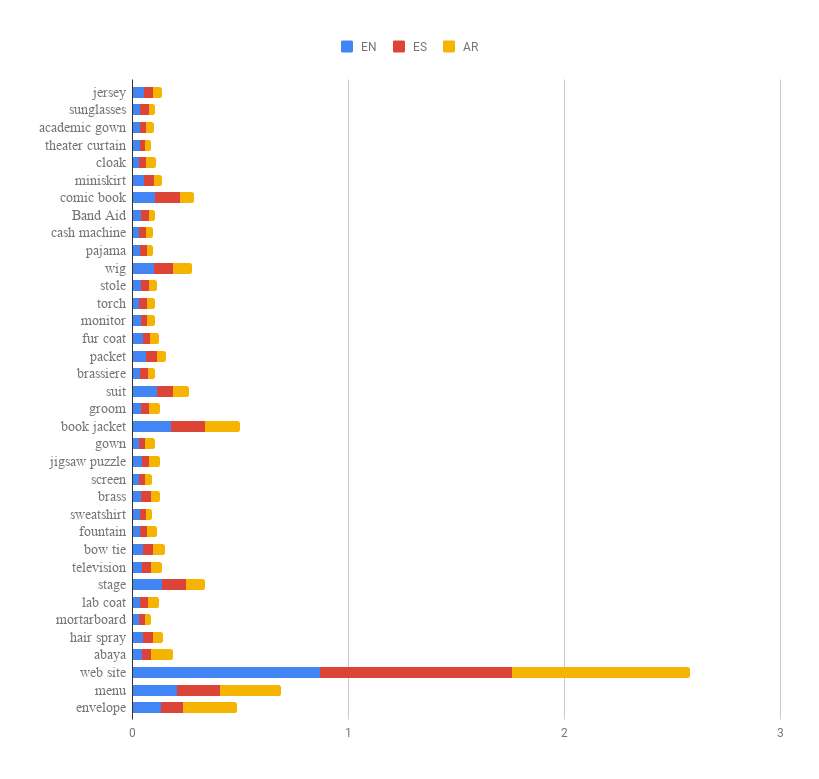
\includegraphics[width=6cm,height=7cm]{img/females_most_freq.png}}
\subfloat[Males most frequent attributes.]{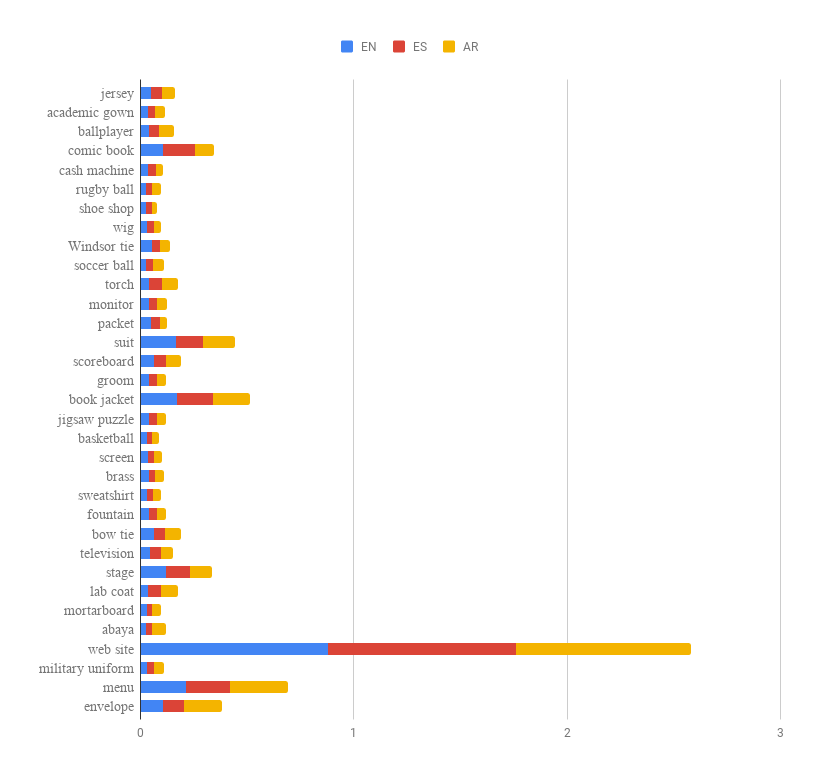
\includegraphics[width=6cm,height=7cm]{img/males_most_freq.png}}
\caption{Intersection of the 50 highest value features of the normalized sum vectors for every language.}
\label{img-vgg16-freqs}
\end{figure}

Furthermore, we use every possible pair of the normalized sum vectors
to compute the Jaccard index between 
them. We extend the number of 50 attributes to 100 for
each normalized sum vector. We use the Jaccard index to measure similarity between the
100 features of the sum vector with the highest values. Tables \ref{table:women-vs-women-and-men-vs-men} and \ref{table:women-vs-men} show
the results.
%Los Cuadros \ref{table:men-vs-men}, \ref{table:women-vs-women}, \ref{table:women-vs-men} muestran los resultados.
%En relación a los valores de los coeficientes de correlación, se 
%puede ver que los mismos Genders en diferentes Languages tienen
%valores muy altos. Sin embargo, también Genders diferentes en distintos
%Languages tienen una fuerte correlación. Con base en lo anterior, se puede
%deducir que existen sólo algunos atributos sobre los que
%recae la representación del Gender de los autores.

% We use the Jaccard index to measure similarity between the
% 100 features of the sum vector with the highest values.
% Tables \ref{table:men-vs-men}, \ref{table:women-vs-women} and \ref{table:women-vs-men} shows a better perspective with respect to the correlation measure. 


\begin{table}[!htb]
    \caption{Jaccard index between every pair of males (table on the left) and between every pair of females (table on the right).}
    \label{table:women-vs-women-and-men-vs-men}
    \begin{minipage}{.5\linewidth}
        \centering
        \begin{tabular}{ll}
        \hline
                        & Jaccard index \\ \hline
        Arab-Spanish    & 0.681         \\
        Arab-English    & 0.724         \\
        Spanish-English & 0.739         \\ \hline
        \end{tabular}
    \end{minipage}%
    \begin{minipage}{.5\linewidth}
        \centering
        
        \begin{tabular}{ll}
        \hline
                        & Jaccard index \\ \hline
        Arab-Spanish    & 0.667         \\
        Arab-English    & 0.653         \\
        Spanish-English & 0.802         \\ \hline
        \end{tabular}
    \end{minipage} 
\end{table}


\begin{table}[!htb]
    \centering
    \caption{Jaccard index (right) between males and females.}
    \label{table:women-vs-men}
    \begin{tabular}{@{}llll@{}}
    \toprule
    \diagbox{Males}{Females} & Arab  & Spanish & English \\ \midrule
    Arab                     & 0.626 & 0.626   & 0.613   \\
    Spanish                  & 0.563 & 0.681   & 0.667   \\
    English                  & 0.550 & 0.587   & 0.626   \\ \bottomrule
    \end{tabular}
\end{table}

We can see
that the pairs of most similar sets are: english with arab-speaking males, english with spanish-speaking males
and  english with spanish speaking females. Conversely, 
the least similar are between males and females
from the pair of languages: spanish and arab, english and arab, spanish and english. 
We can also see from Table \ref{table:women-vs-women-and-men-vs-men} that there is more dissimilarity with respect to arab users. We can assume that it is due to a wider cultural gap than among the english and spanish-speaking users. Motivated by knowing what kind of things those
makes those users uniques, we compute the difference between the
sum vector of the arab users and the average sum vector of spanish and
english users. Figure  \ref{img-arab-comparison} shows those attributes
not to close to zero, where attributes with negative values are less 
prevalent in images of arab-speaking users and those positives are
more common.

\begin{figure}[h]
\centering
\subfloat[Arab females comparison with other speaking user languages. ]{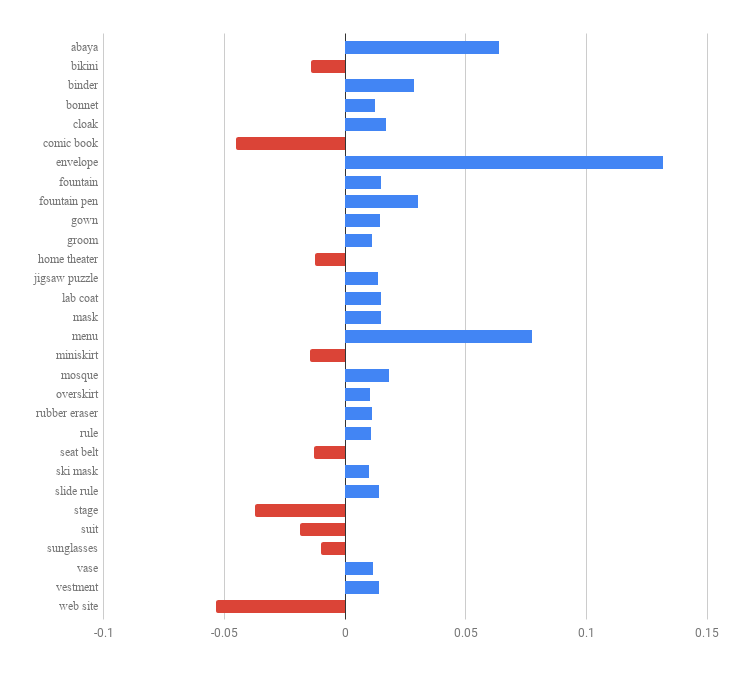
\includegraphics[scale=0.23]{img/ar_females_vs_all.png}}
\subfloat[Arab males comparison with other speaking user languages.]{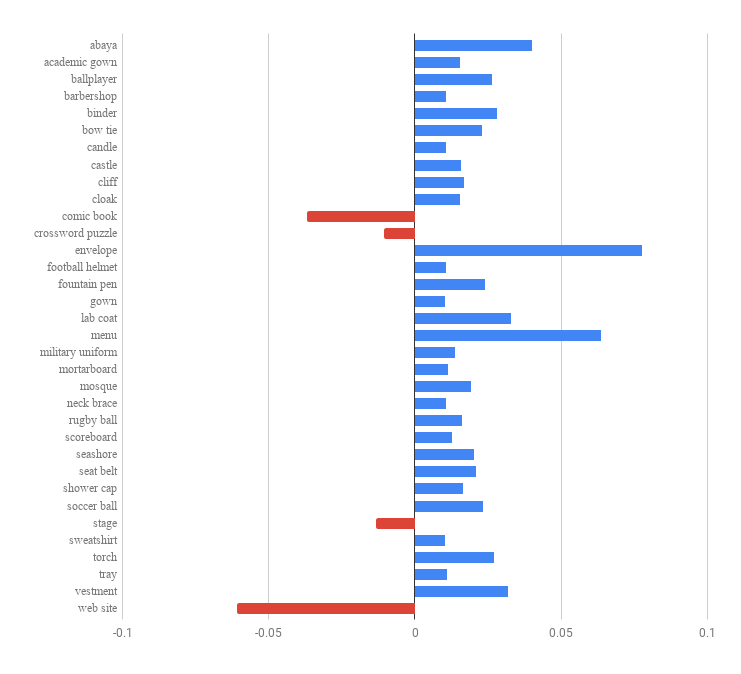
\includegraphics[scale=0.23]{img/ar_males_vs_all.png}}
\caption{Difference between arab-speaking users and the others.}
\label{img-arab-comparison}
\end{figure}


%
%
%
%Con respecto al Jaccard index para medir la similitud entre los conjuntos
%de tamaño 100 de atributos entre los diferentes Languages y Genders se puede 
%ver que los pares de conjuntos más similares son entre Males de los
%Languages: inglés - arabe e inglés - español y entre Females de español - inglés. Por el contrario,
%los conjuntos menos similares son entre Males y Females de los Languages:
%español - árabe, inglés - árabe y español - inglés.

% {'hair_spray', 'brassiere', 'stole', 'Blenheim_spaniel', 'Persian_cat', 'overskirt', 'miniskirt', 'ballplayer', 'velvet', 'lipstick', 'wig', 'bath_towel', 'Shih-Tzu', 'spatula', 'suit'}


% \begin{table}[]
% \centering
% \caption{Correlation and Jaccard index from males of every language.}
% \label{table:men-vs-men}
% \begin{tabular}{@{}lll@{}}
% \toprule
%                 & \begin{tabular}[c]{@{}l@{}}Correlation \\ coefficient\end{tabular} & Jaccard index \\ \midrule
% Arab-Spanish    & 0.985                                                             & 0.681         \\
% Arab-English    & 0.986                                                             & 0.724         \\
% Spanish-English & 0.996                                                             & 0.739         \\ \bottomrule
% \end{tabular}
% \end{table}
% \begin{table}[]
% \centering
% \caption{Correlation and Jaccard index from males of every language.}
% \label{table:men-vs-men}
% \begin{tabular}{|l|l|l|}
% \hline
% & \begin{tabular}[c]{@{}l@{}}Correlation \\ coeficient\end{tabular} & Jaccard index \\ \hline
% Arab-Spanish              & 0.985                                                                 & 0.681          \\ \hline
% Arab-English               & 0.986                                                                 & 0.724          \\ \hline
% Spanish-English             & 0.996                                                                 & 0.739          \\ \hline
% \end{tabular}
% \end{table}


% \begin{table}[]
% \centering
% \caption{Correlation and Jaccard index from females of every language.}
% \label{table:women-vs-women}
% \begin{tabular}{@{}lll@{}}
% \toprule
%                 & \begin{tabular}[c]{@{}l@{}}Correlation \\ coefficient\end{tabular} & Jaccard index \\ \midrule
% Arab-Spanish    & 0.973                                                             & 0.667         \\
% Arab-English    & 0.976                                                             & 0.653         \\
% Spanish-English & 0.997                                                             & 0.802         \\ \bottomrule
% \end{tabular}
% \end{table}

% \begin{table}[]
% \centering
% \caption{Correlation and Jaccard index from fesmales of every language.}
% \label{table:women-vs-women}
% \begin{tabular}{|l|l|l|}
% \hline
% & \begin{tabular}[c]{@{}l@{}}Correlation \\ coeficient\end{tabular} & Jaccard index \\ \hline
% Arab-Spanish   & 0.973                      & 0.667          \\ \hline
% Arab-English    & 0.976                      & 0.653          \\ \hline
% Spanish-English  & 0.997                      & 0.802          \\ \hline
% \end{tabular}
% \end{table}

% \begin{table}[!htb]
%     \caption{Correlation (left) and Jaccard index (right) between males and females.}
%     \label{table:women-vs-men}
%     \begin{minipage}{.5\linewidth}
%         \centering
%         \begin{tabular}{@{}llll@{}}
%         \toprule
%         \diagbox{Males}{Females} & Arab  & Spanish & English \\ \midrule
%         Arab                     & 0.982 & 0.977   & 0.980   \\
%         Spanish                  & 0.962 & 0.990   & 0.990   \\
%         English                  & 0.964 & 0.987   & 0.991   \\ \bottomrule
%         \end{tabular}
%     \end{minipage}%
%     \begin{minipage}{.5\linewidth}
%         \centering
        
%         \begin{tabular}{@{}llll@{}}
%         \toprule
%         \diagbox{Males}{Females} & Arab  & Spanish & English \\ \midrule
%         Arab                     & 0.626 & 0.626   & 0.613   \\
%         Spanish                  & 0.563 & 0.681   & 0.667   \\
%         English                  & 0.550 & 0.587   & 0.626   \\ \bottomrule
%         \end{tabular}
%     \end{minipage} 
% \end{table}




To expand the sum-based analysis we also try a feature selection
technique to get those attributes that help in the distinction of 
gender in each language. We compute for each language collection the 
information gain for every attribute. 
% Figure \ref{img-gi} indicates, through Venn diagrams, the 25 attributes (for viewing reasons) with greater information gain for every pair of languages. 
% Further, t
The terms that comprise the intersection of the three sets of 100 features with higher information gain are: hair spray, brassiere, stole, blenheim spaniel, persian cat, over skirt, miniskirt, ballplayer, velvet, lipstick, wig, bath towel, shih tzu, spatula and suit.

For a better visualization of the content shared by users we 
choose two attributes, bath towel and ballplayer and select some of the images from different users. They are displayed in
Figures \ref{fig:towel} and \ref{fig:ballplayer}.

% El otro análisis se realizó con una perspectiva 
% de selección de atributos, obteniendo la ganancia de información 
% de los atributos en cada Language. En la Figura \ref{img-gi} se muestran diagramas con los 25 atributos con mayor ganancia de información para cada par de Languages. 
% La intersección de los 25 atributos para los tres conjuntos de Languages 
% son cuatro: brassiere}, lipstick}, velvet} y 
% bath towel}. A partir de estas cuatro características importantes
% se realizó un análisis de fotografías cuyos valores sobre esos atributos
% fueron altos. De las Figuras \ref{fig:towel}, \ref{fig:brassiere}, 
% \ref{fig:lipstick}, \ref{fig:velvet} se puede ver las imágenes compartidas
% y el resultado de los modelos de identificacióń de Gender, el cual fue el Gender
% Female utilizando todos lo modelos, excepto en una fotografía en la que dos modelos,
% el entrenado con inglés y árabe y el monolingüe inglés, identificaron al autor
% como Male.

% Al aumentar la lista a las 100 características con mayor ganancia de información
% se consigue una intersección mayor entre los tres Languages. La intersección
% de atributos para 100 características es: hair spray}, brassiere}, stole}, Blenheim spaniel}, Persian cat}, overskirt}, miniskirt}, ballplayer}, velvet}, lipstick}, wig}, bath towel}, Shih Tzu}, spatula} y suit}.

% Se realizó el mismo experimento de obtener imágenes que tienen una alta 
% probabilidad de contener la característica ballplayer}, para
% observar a qué Gender permitía distinguir. En la Figura \ref{fig:ballplayer}
% se muestran los resultados para los diferentes Languages, el Gender identificado
% fue el Male.


% \begin{figure}[ht]
% \centering
% \subfloat[English $\cap$ Spanish]{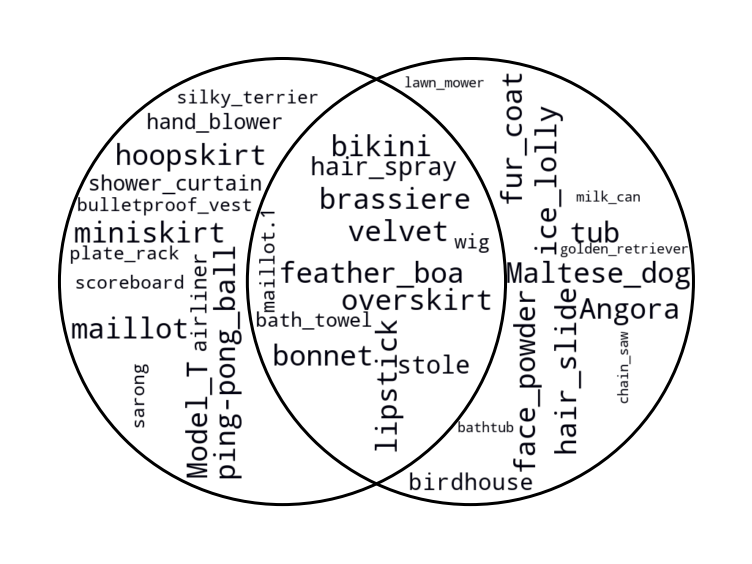
\includegraphics[scale=0.24]{img/en_es_gi.png}}
% \subfloat[English $\cap$ Arab]{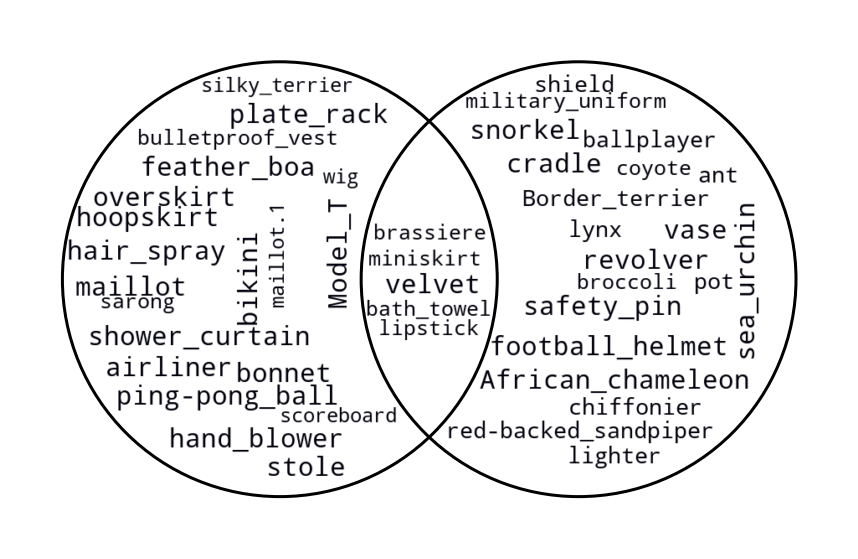
\includegraphics[scale=0.24]{img/en_ar_gi.png}}\\
% \subfloat[Spanish $\cap$ Arab]{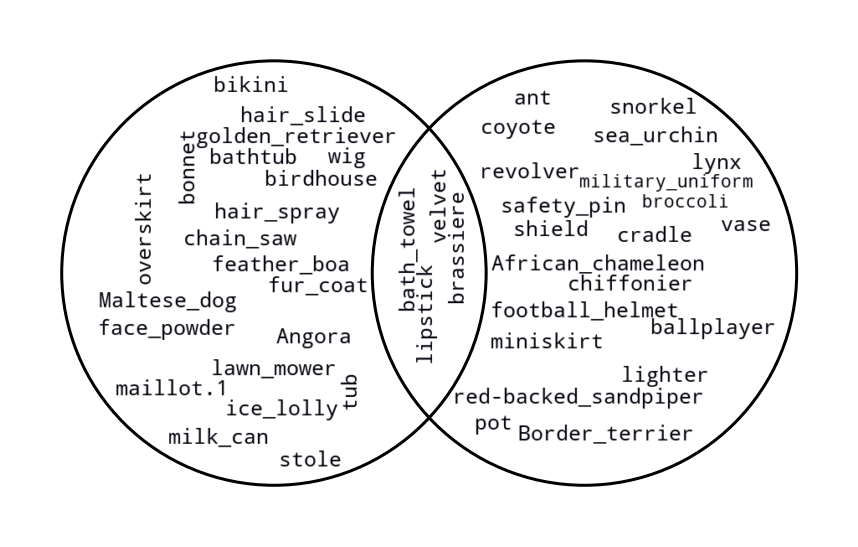
\includegraphics[scale=0.24]{img/es_ar_gi.png}}   
% \caption{Venn diagrams for the 25 attributes with greater information
% gain.}
% \label{img-gi}
% \end{figure}



\begin{figure}[!ht]
    \centering
    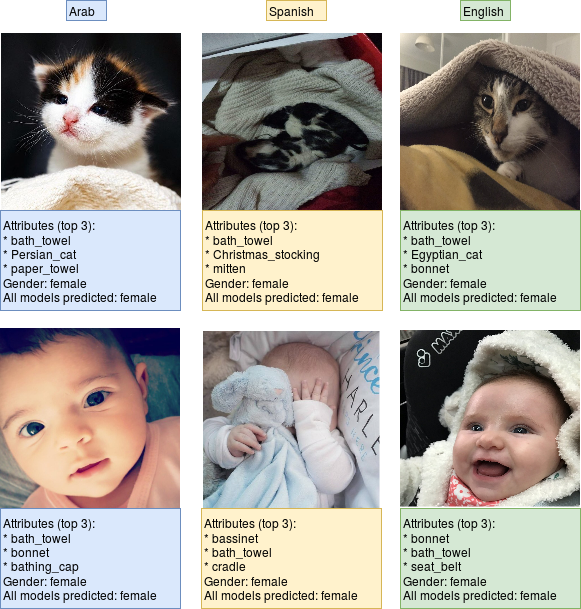
\includegraphics[scale=0.37]{img/best_gi/bath_towel_gi.png}
    \caption{Bath towel.}
    \label{fig:towel}
\end{figure}
% \begin{figure}[ht]
%     \centering
%     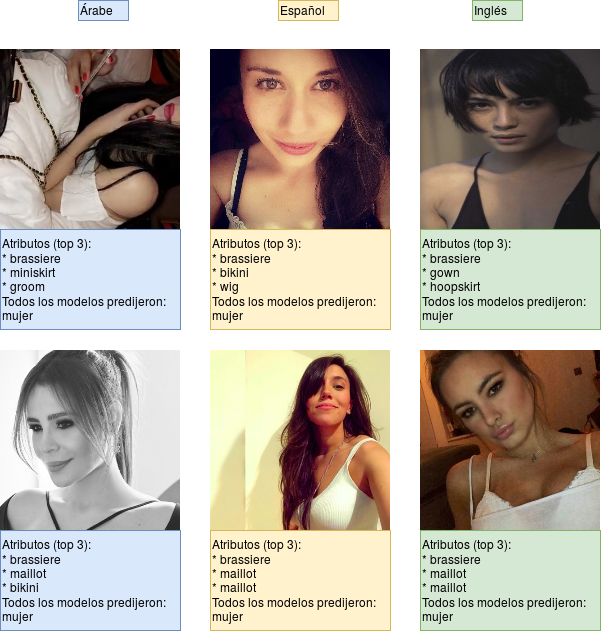
\includegraphics[scale=0.37]{img/best_gi/brassiere_gi.png}
%     \caption{Brassiere.}
%     \label{fig:brassiere}
% \end{figure}
% \begin{figure}[ht]
%     \centering
%     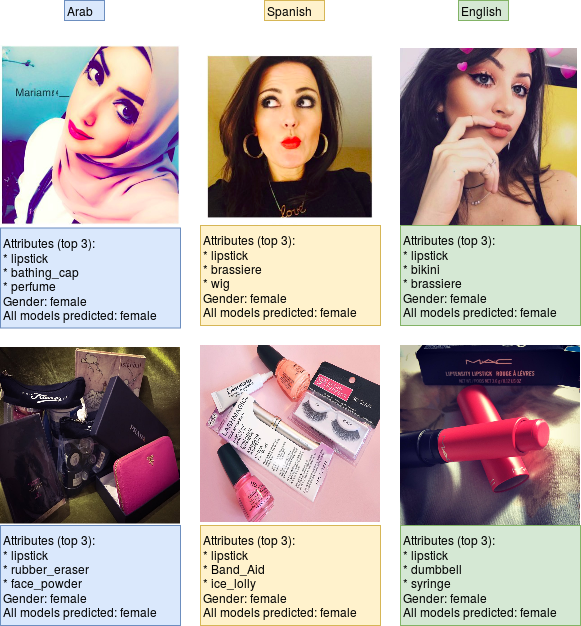
\includegraphics[scale=0.37]{img/best_gi/lipstick_gi.png}
%     \caption{Lipstick.}
%     \label{fig:lipstick}
% \end{figure}
% \begin{figure}[ht]
%     \centering
%     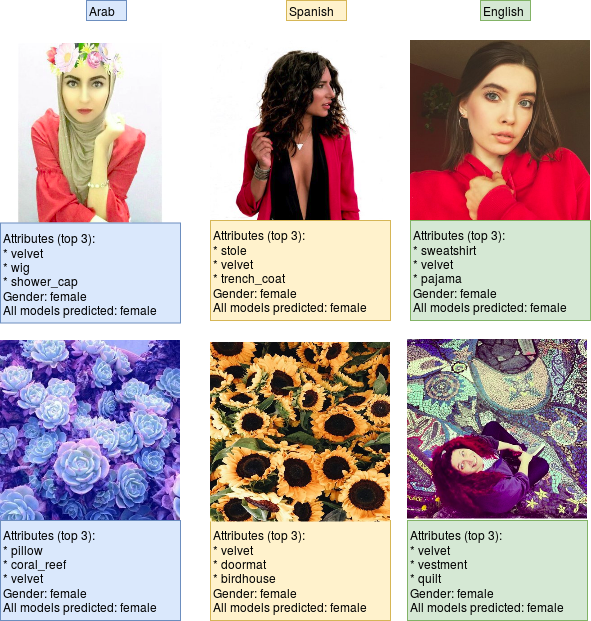
\includegraphics[scale=0.37]{img/best_gi/velvet_gi.png}
%     \caption{Velvet.}
%     \label{fig:velvet}
% \end{figure}
\begin{figure}[!ht]
    \centering
    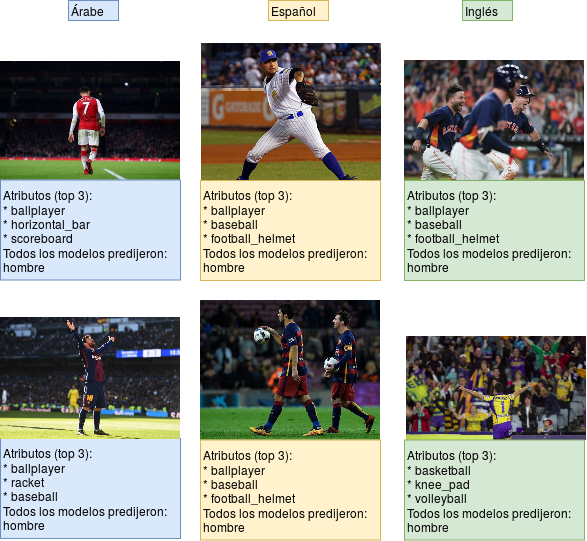
\includegraphics[scale=0.37]{img/best_gi/ball_player_gi.png}
    \caption{Ballplayer.}
    \label{fig:ballplayer}
\end{figure}
% \begin{itemize}
%     \item Análisis de resultados.
%     \item Tablas de las combinaciones que se probaron.
%     \item Selección de características.
%     \item Histogramas de ``frecuencias''.
%     \item Correlación entre los vectores de los Males y Females
%     entre los Languages.
% \end{itemize}

\newpage
\section{Conclusions and future work}
In this paper, we proposed a cross-cultural image-based approach for gender prediction in social media.
This scheme was evaluated over a collection of Twitter images
from users of three different languages. The results 
have proven that the content of the images 
among the users is independent of the user language,
i.e. males from different languages
tend to share the same type of images between different languages, same happens with female users. This work shows that cultural and language barriers have been overcome among users of social networks.
A direction of future work is to try to achieve state of the art results from text or other image based approaches. Some of the proposals for the future is to improve authors representations
using more abstract features or put the one thousand labels into higher level batches of categories.


% A partir de los resultados obtenidos, se puede ver un 
% ligero incremento en la exactitud utilizando todas las colecciones para
% entrenar un modelo y probarlo con un Language por separado.
% Además de esto, a través de un análisis de las representaciones
% de las imágenes usando atributos semánticos se pudo observar que hay 
% atributos importantes para distinguir las clases que coinciden en 
% los tres Languages. Sin embargo, a pesar de que el desempeño obtenido es bueno,
% está por debajo del que obtuvieron los autores en \cite{takahashi_tahara_nagatan_miura_taniguchi_ohkuma} que obtuvo
% un promedio de 0.7872, el promedio de nuestros mejores clasificadores fue 
% de 0.6966. Una posible causa es la limitación de nuestra representación
% de cada autor.
% \begin{itemize}
%     \item ¿El Language importa? 
%     \item ¿Comparten lo mismo los usuarios del Gender $X$ en el Language
%     $Y$ y los usuarios del Gender $X$ en el Language $\hat{Y}$.
%     \item ¿Es suficiente el vocabulario con el que cuenta imagenet
%     (1000 objetos y escenarios)?
%     \item Extender el trabajo usando el enfoque no supervisado.
%     \item Vocabulario abierto.
%     \item Agrupamiento dentro de cada Gender.
% \end{itemize}

\bibliographystyle{splncs04}
\bibliography{references}

\end{document}
